 \section{Entwicklung des Formularsystems}

\subsection{Einleitung}

Das Projekt umfasst die strukturierte und DSGVO-konforme Erfassung von Gästedaten mittels einer benutzerfreundlichen Webanwendung für Mieter. Im Fokus steht die Entwicklung eines intuitiven und länderspezifischen Formularsystems, das die Vollständigkeit und Validierung der erfassten Daten sicherstellt, bevor diese an das Backend geliefert werden.
Daraus ergibt sich folgende zentrale Forschungsfrage:

\begin{quote}
\textbf{Wie kann die Erfassung und Verarbeitung von Formulardaten in einer Webanwendung gestaltet werden, sodass die Eingabe effizient, sicher und benutzerfreundlich gewährleistet wird?}
\end{quote}

Das Beantworten dieser Frage setzt die Analyse der derzeitig gängigen Ansätze zur Datenvalidierung und zum Interface-Design voraus. Diese Analyse wird sich hauptsächlich mit der Theorie dieser Ansätze auseinandersetzen.

\subsection{Grundlagen von Formularsystemen}
\subsubsection{Definition und Zweck eines Formulars}
Wie auf Seite zwei des Artikels ''An extensive guide to web form usability'' \cite{mifsud2011extensive} definiert sind Formulare strukturierte Schnittstellen zur Datenerfassung und anschließender Übertragung zwischen Benutzer und Systemen. Sie bestehen im Normalfall aus folgenden Komponenten: \cite{prompt2_pollak}

\begin{enumerate}

    \item \textbf{Labels/Beschriftungen} Sie geben dem Benutzer Kontext und Anweisungen für jedes Eingabefeld.
    
    \item \textbf{Eingabefelder} Eingabefelder ermöglichen, dem Benutzer Informationen bereitzustellen. Dies beinhaltet Textfelder, Passwortfelder, Kontrollkästchen, Optionsschaltflächen, Schieberegler und mehr.
    
    \item \textbf{Action} Aktionen geben dem Benutzer die Möglichkeit, mittels eines Buttons oder Links eine Aktion durchzuführen, wie zum Beispiel das Absenden des Formulars.

    \item \textbf{Help} Die Hilfefunktion soll den Benutzer dabei unterstützen, das Formular korrekt auszufüllen, indem sie beispielsweise eine Erklärung zu einem Eingabefeld liefert, wie in Abbildung \ref{fig:abbildung2} dargestellt.
    
    \item \textbf{Messages} Nachrichten geben dem Benutzer Rückmeldung basierend auf seinen Eingaben. Diese können positiv sein (zum Beispiel, dass das Formular erfolgreich übermittelt wurde) oder negativ („Der von Ihnen gewählte Benutzername ist bereits vergeben“).

    \item \textbf{\gls{form-validation}} Das Validieren der Daten stellt sicher, dass die vom Benutzer übergebenen Daten den Akzeptanzkriterien entsprechen. Auf Datenvalidierung wird im Kapitel \ref{datenvaliderung} genauer eingegangen.
    
\end{enumerate}

\begin{figure}
    \centering
    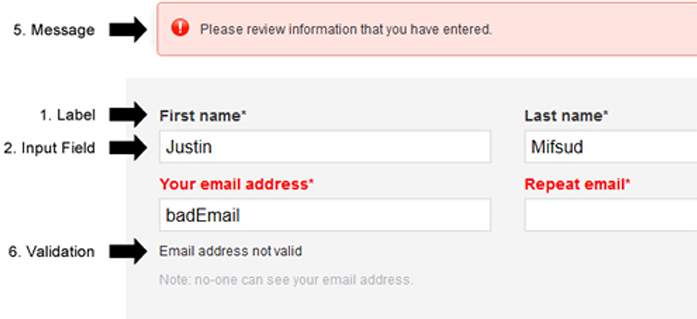
\includegraphics[width=0.75\linewidth]{images/formularKomponenten1.png}
    \caption{Formularkomponenten 1 \cite{mifsud2011extensive}}
    \label{fig:abbildung1}
\end{figure}

\begin{figure}
    \centering
    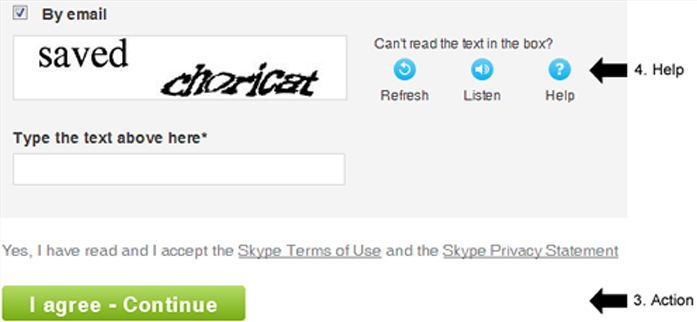
\includegraphics[width=0.75\linewidth]{images/formularKomponenten2.png}
    \caption{Formularkomponenten 2 \cite{mifsud2011extensive}}
    \label{fig:abbildung2}
\end{figure}

Wie im ersten Kapitel des Buches ''Web form design: Filling in the blanks'' \cite{wroblewski2008web} nachgelesen werden kann, bieten Formulare sowohl aus der Perspektive des Benutzers als auch des Anbieters allerlei Vorteile. Sie steigern generell die Effizienz und verbessern die \gls{usability}. Sie strukturieren Daten in einem vordefinierten Format und leiten die Benutzer bei guter Gestaltung effektiv durch den Eingabeprozess. Ebenso wird, wie oberhalb erwähnt, die Integrität der Daten sichergestellt, was wichtig ist, um eine potenzielle Prozessautomatisierung zu ermöglichen.

\subsubsection{Historische Entwicklung}
Die Geschichte der Formulare beginnt mit handgeschriebenen Dokumenten auf Papier. Diese frühen Formulare dienten der strukturierten Erfassung von Informationen, um Verwaltungsprozesse zu optimieren. Nachdem in den 1990er Jahren das World Wide Web mit statischen Seiten entstanden war, wuchs der Wunsch der Nutzer, aktiv zu interagieren und nicht nur Informationen zu konsumieren. Infolgedessen wurden die oben beschriebenen Formulare entwickelt. Diese ermöglichten dann erstmals die Datenerfassung über den Webbrowser. Dies beschreiben Caroline Jarrett und Gerry Gaffney in ihrem Buch ''Forms that work: Designing web forms for usability'' \cite{jarrett2009forms}. \cite{prompt3_pollak}

\subsection{\gls{usability} und Formulardesign}
\subsubsection{Warum ist das Formulardesign wichtig?}
Formulare stehen immer zwischen dem Ziel des Benutzers und den Zielen der Firmen. Beispielsweise möchten Kunden auf E-Commerce-Websites Dinge kaufen, die sie brauchen, und das Unternehmen möchte den Umsatz maximieren. Im Weg steht dabei das Checkout-Formular.
Daher ist es in diesem Beispiel wichtig, das Checkout-Formular besonders benutzerfreundlich zu gestalten. Wie im ersten Kapitel des Buches ''Web form design: Filling in the blanks'' \cite{wroblewski2008web} aufzeigt, kann durch diese Optimierung die Anzahl erfolgreich abgeschlossener Check-outs oder Registrierungen je nach Anwendungsfall um 10 bis 40 Prozent gesteigert werden.
 \cite{prompt4_pollak}

\subsubsection{Prinzipien des Userinterface Designs für Formulare}
Da das Formulardesign Abschluss- und Fehlerraten stark beeinflusst, stellt sich die Frage: Wie designt man gute Formulare? Auf diese Frage gibt es leider keine universelle Antwort, da diese von den Geschäfts- und Nutzerzielen sowie vom Kontext abhängt. Folgende Theorie können jedoch zur Umsetzung beitragen:

In dem Buch ''Forms that Work: Designing Web Forms for Usability'' \cite[S. 5-6]{jarrett2009forms} von Caroline Jarrett und Gerry Gaffney wird eine Theorie beschrieben, die besagt, dass ein Formular immer aus den drei folgenden Ebenen besteht.
\begin{enumerate}
    \item \textbf{Beziehung} Formulare etablieren eine Beziehung zwischen dem Nutzer und der Organisation.
    
    \item \textbf{Konversation} Sie ermöglichen einen Dialog zwischen dem Nutzer und der Organisation.
    
    \item \textbf{Visuelle Ebene} Durch ihr Aussehen prägen sie sowohl die Beziehung als auch die Konversation.
\end{enumerate}
Auf den Benutzer wirken immer alle drei Ebenen gemeinsam. Um ein Formular wirklich benutzerfreundlich zu gestalten, müssen alle drei berücksichtigt werden.

Um die praktische Anwendung des oben erklärten Konzepts zu verdeutlichen, ist eine detaillierte Untersuchung jeder einzelnen Ebene hilfreich. Im Folgenden wird sich mit den charakteristischen Aspekten jeder dieser Ebenen auseinandergesetzt. \cite{prompt5_pollak}

\paragraph{Beziehung}
Bei dem Stellen einer Frage in einem Formular wird eine Antwort erwartet. Dies stellt für den Benutzer eine Investition dar. Die Quantität bzw. die Qualität der erhaltenen Antwort hängt stark von der derzeitigen Beziehung zur Organisation ab. Diese Beziehung kann von folgenden Faktoren abhängen:
\begin{enumerate}
    \item \textbf{Vertrauen} Vertrauen ist essenziell für eine solche Beziehung. Dies kann erreicht werden durch Seriosität. 
    
    \item \textbf{Relevanz der Fragen} Formulare sind in einem spezifischen Rahmen zu finden. Die Berücksichtigung von Zielgruppe, Anwendungsfall und Geschäftszielen optimiert die Akzeptanz. 
     
    \item \textbf{Konsistenz} Auch wenn verschiedene Abteilungen (z. B. Marketing, Datenschutz, Technik, Design) daran mitwirken, soll das Formular konsistent wirken. Bei nicht Einhalten der Konsistenz kann das Formular Misstrauen hervorrufen.
\end{enumerate} 

\paragraph{Konversation}
Ein Formular ist in gewisser Hinsicht eine Konversation zwischen dem Nutzer und der Organisation. Eine Konversation zeichnet sich durch bestimmte Aspekte aus:
\begin{enumerate}

    \item \textbf{Tonfall} Das Formular sollte keine aggressive oder abschreckende Atmosphäre schaffen. 
    
    \item \textbf{Logische Struktur und Fluss} Eine Konversation hat eine logische sinnvollen Gesprächsstruktur. Dies sollte ebenso bei einem Formular der Fall sein.
    
    \item \textbf{Klare Handlungsanweisungen} Da das Ziel eines Formulars das Ausfüllen ist, sollte möglichst klar beschrieben werden, wie dies erreicht werden kann.
    
\end{enumerate}

\paragraph{Visuelle Ebene}
Bisher wurde sich nur mit den tieferen Aspekten beschäftigt. Jetzt wird sich auf das Aussehen konzentriert. Das richtige Platzieren von Komponenten und das professionelle Auftreten sind essenziell für ein gelungenes Formular. Folgend wird grob darauf eingegangen, wie dies umgesetzt werden kann:
\begin{enumerate}
    \item \textbf{Labels}
    Die Position von Labels kann Auswirkungen auf Lesegeschwindigkeit und Nutzerfreundlichkeit haben. Für optimale Lesegeschwindigkeit sollten sie oberhalb platziert werden. Die Labels können auch links neben dem Eingabefeld platziert werden. Alle anderen Seiten sollten vermieden werden.
    
    \item \textbf{Struktur}
    Das Formular sollte klar strukturiert sein. Wichtig dabei sind Gruppierungen von zusammenhängenden Fragen in logische Themenbereiche. Dazu können dezente Linien verwendet werden. Jedoch sollten keine kreativen oder verspielten Designs verwendet werden. Ein zweispaltiges Layout sollte vermieden werden, da dies zu Verwirrung führen kann.
    
    \item \textbf{Konsistenz und Styleguide}
    Wichtig für ein seriöses Auftreten ist die visuelle Konsistenz. Dabei kann ein Styleguide helfen, um den Stil über alle Formulare hinweg zu wahren. In diesem können Schriftarten und die Art von Labels definiert werden. Es sollte sich auch an eine einheitliche Gruppierungslogik gehalten werden.
    
    \item \textbf{Vertrauensaufbau durch Design}
    Vertrauen hängt in erster Linie von einem seriösen Design ab. Das kann mit den oberen Punkten gewährleistet werden, jedoch ist es auch wichtig, dass das Formular klar zeigt, wer der Anbieter ist und was mit den Daten passiert.
\end{enumerate}

\subsection{Datenvalidierung und Vollständigkeitsprüfung \label{datenvaliderung}}
\subsubsection{Definition und Zweck von Datenvalidierung}
Datenvalidierung sorgt im Allgemeinen für die Prüfung der Benutzereingaben auf ihre Gültigkeit und Plausibilität. Durch nicht validierte Daten können Programmfehler und Sicherheitsprobleme entstehen. Bei der Datenvalidierung wird überprüft, ob Werte zu einem bestimmten Datentyp gehören oder in einem vorgegebenen Wertebereich liegen, siehe dem Wikipedia Artikel ''Datenvalidierung'' \cite{wikiDatavalidation}. Bei der Validierung von Benutzereingaben sollten immer folgende zwei Prinzipien beachtet werden:

\begin{enumerate}

    \item \textbf{Never Trust the User} Hiermit ist gemeint, dass dem Benutzer nie vertraut werden soll und daher immer alle Benutzereingaben validiert werden müssen.
    
    \item \textbf{Fail-Fast} Bei Fail-Fast sollte zur Laufzeit sofort ein Fehler geworfen werden, falls falschen Parameterwerte übergeben werden. Damit werden kompliziertere Folgefehler vermieden.
    
\end{enumerate}

\paragraph{Warum ist Datenvalidierung wichtig?}
Datenvalidierung ist in Hinsicht auf zwei Aspekte wichtig. Erstens in Hinsicht auf den Nutzer und zweitens in Hinsicht auf die Sicherheit. Folgend wird genauer auf diese Aspekte eingegangen. \cite{prompt6_pollak}

\paragraph{Nutzerzentrierte Datenintegrität}
Bei korrekter Datenvalidierung kann der Nutzer nur valide Daten übergeben. Bei fehlerhafter Eingabe bekommt der Nutzer Feedback, was falsch gemacht wurde. Dadurch wird die Integrität der Daten gewährleistet. Infolgedessen kommt es zu weniger bis gar keinen Fehlern bei der Verarbeitung. Ein Beispiel hierfür wäre das Eingabefeld für eine E-Mail-Adresse. Wenn diese auf syntaktische Korrektheit geprüft wird, können keine Fehler mehr beim Versenden von E-Mails geschehen (ausgenommen eines semantischen Fehlers).

\paragraph{Sicherheit}
\label{sec:sicherheit}
Der zweite wichtige Aspekt der Datenvalidierung ist laut dem Paper ''A modular approach to data validation in web applications'' \cite{DeVries2006} der Schutz vor Sicherheitsrisiken. Bei fehlerhafter Datenvalidierung könnten Angreifer die Funktionsweise des Systems umgehen, unbefugte Befehle ausführen oder Code auf Backend-Systemen einschleusen. Beispiele dafür wären folgende Attacken:

\begin{enumerate}

    \item \textbf{Parameter Manipulation} Eine Sicherheitslücke, die entsteht, wenn das Backend clientseitig übermittelte Parameter als vertrauenswürdig behandelt. Somit können Angreifer die übermittelten Parameter verändern und damit die Anwendung manipulieren. \cite{prompt7_pollak}
    
    \item \textbf{Code Injection} Bei Code Injections versuchen Angreifer Daten als Befehle zu übergeben. Daher ist die Unterscheidung zwischen Daten und Befehlen wichtig, siehe Kapitel 3\cite{DeVries2006}. \cite{prompt8_pollak} \cite{prompt9_pollak}
    
\end{enumerate}

\subsubsection{Prinzipen von Datenvalidierung}
Folgend wird sich damit beschäftigt, wie die Validierung umgesetzt werden kann und welche Prinzipien dabei beachtet werden, basierend auf den Empfehlungen des oben genannten Papers \cite{DeVries2006}.
    
\paragraph{Reduktion auf eine standardisierte Form}
Bevor Daten verarbeitet werden, sollten diese auf ihre einfachste beziehungsweise auf eine einheitliche Form gebracht werden. Dies kann geschehen, indem die Daten in ASCII, Unicode, UTF-8 oder andere umgewandelt werden. Wenn die Anwendung die Daten vor der Validierung nicht korrekt dekodiert, sind diese weitgehend nutzlos. Dies kann dazu führen, dass fehlerhafte oder schädliche Daten das Backend erreichen.
 
\paragraph{Rejektion invalider Daten}
Bei dieser Art der Validierung werden alle ungültigen Daten blockiert, indem eine Liste möglicher fehlerhafter oder unerwünschter Eingaben erstellt wird. Daten, die auf diese Liste passen, werden abgelehnt. In den meisten Fällen ist dieser Ansatz jedoch nicht ideal, da es sehr schwierig ist, eine solche Liste vollständig und fehlerfrei zu erstellen, um alle möglichen Risiken zuverlässig abzudecken.

\paragraph{Akzeptanz verifizierter Eingaben}
Das Pendant dazu ist die Art der Validierung, bei der nur Daten akzeptiert werden, die genau den Kriterien entsprechen. Hier wird ebenso eine Liste verwendet, auf der alle erlaubten Kriterien festgehalten wurden. Dies ist einfacher umzusetzen und bietet im Normalfall eine erhöhte Sicherheit. Bei diesem Prinzip besteht jedoch das Problem mit Sonderzeichen. Diese können als valide Daten definiert sein, jedoch können sie auch zu Problemen in Hinsicht auf Sicherheit führen, siehe Code Injections \ref{sec:sicherheit}.

\paragraph{Datenbereinigung}
Diese Variante ist die Kombination der beiden oberen Validierungsmethoden. Hier werden alle ungültigen Daten blockiert und nur Daten akzeptiert, die genau den Kriterien entsprechen. Damit kann das Problem der Sonderzeichen beinahe beseitigt werden.  

\paragraph{Ort der Datenvalidierung}
Wie man in Kapitel 5 des Papers \cite{DeVries2006} nachgelesen werden kann, muss die Datenvalidierung in Hinsicht auf die Sicherheit immer auf dem Server stattfinden, da dem Code auf der Seite des Clients nie vertraut werden darf. Diese kann immer manipuliert werden. Nutzerorientierte Datenvalidierung jedoch kann beim Client passieren. Diese ist nicht immer sicherheitsrelevant und ebenso kann das Feedback an den Benutzer leichter verarbeitet werden. 

\subsection{Ergebnis der Literaturrecherche}
Diese Ausarbeitung verdeutlicht die wesentlichen Prinzipien und Ansätze für die Entwicklung eines Formularsystems in Hinsicht auf \gls{usability} und Datenvalidierung. Die Analyse der Benutzerfreundlichkeit verdeutlichte die Bedeutung eines gut durchdachten Designs und was bei diesem bedacht werden sollte. 

Zusätzlich wurde hervorgehoben, dass die Datenvalidierung ein zentrales Element ist, um sowohl die Integrität der erfassten Informationen als auch die Systemsicherheit zu gewährleisten.

Die gewonnenen Erkenntnisse sind Grundlage für die Umsetzung eines benutzerfreundlichen und sicheren Formularsystems. Damit bietet diese Arbeit nicht nur einen wertvollen Beitrag für das Projekt, sondern es wurde eine Basis gelegt, um auch die zentrale Forschungsfrage zu beantworten. \cite{prompt10_pollak} \cite{prompt1_pollak}